\documentclass[tikz]{standalone}

\usetikzlibrary{positioning, backgrounds,fadings}
\tikzset{background rectangle/.style={fill=white}}
\usepackage{lmodern}
\usepackage{microtype} % for \textls[amount]{text} to reduce spacing between digits
\usepackage{amssymb} % for \maltese character for jokers

\begin{tikzfadingfrompicture}[name=fadingC]
\node[circle,line width=0pt,fill=black!5,draw=black!10,minimum size = 27] at (0,0){};
\end{tikzfadingfrompicture}

\newcommand{\scale}{4.85}

\begin{tikzfadingfrompicture}[name=fadingD]
\node[white] {\scalebox{\scale}{\textbf{+}}};
\end{tikzfadingfrompicture}

\begin{tikzfadingfrompicture}[name=fading777]
\node[white] {\scalebox{2.5}{\textbf{777}}};
\end{tikzfadingfrompicture}

\begin{tikzfadingfrompicture}[name=fadingJ]
\node[white] {\scalebox{\scale}{\textbf{\maltese}}};
\end{tikzfadingfrompicture}

\foreach \x in {1,2,...,9} {
\begin{tikzfadingfrompicture}[name=fading\x]
\node[white] {\scalebox{\scale}{\sffamily\textbf{\x}}};
\end{tikzfadingfrompicture}
}

\foreach \x in {0,1,2,3} {
\begin{tikzfadingfrompicture}[name=fading1\x]
\node[white] {\scalebox{\scale}{\sffamily\textbf{1\hspace{-.36mm}\x}}};
\end{tikzfadingfrompicture}
}

% \scalebox{5}{\textbf{\textcolor{#2}{\textls[-110]{#1}}}} 

\newcommand{\tile}[2]{
    \begin{tikzpicture}[show background rectangle, inner frame sep=0mm]
    \filldraw [rounded corners=4pt, fill=olive!17, draw=olive!33, line width=6pt] (0,0) rectangle (2,3);
    \fill[path fading=fading#1, ball color=#2, shading angle=195] (1,2.1) circle[radius=1];
    \fill[path fading=fadingC, ball color=olive!15, shading angle=300] (1,.75) circle[radius=0.8];
    \end{tikzpicture} 
}

\colorlet{myred}{red!85!black}
\definecolor{myblue}{HTML}{BA55D3}
% \colorlet{myblue}{blue!60!green}
\definecolor{myyellow}{HTML}{FFD700}
\colorlet{mygreen}{green!90!black}
\colorlet{myblack}{black}
\definecolor{extra}{HTML}{FFA500}

\begin{document}

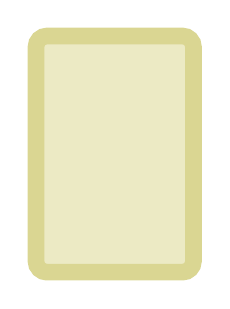
\begin{tikzpicture}[show background rectangle, inner frame sep=0mm]
\filldraw [rounded corners=4pt, fill=olive!17, draw=olive!33, line width=6pt] (0,0) rectangle (2,3);
% \node at (1,2.1) {\scalebox{3}{\textbf{\textls[-80]{\textcolor{myblack}{7}\textcolor{extra}{7}\textcolor{myred}{7}}}}  };
% \fill[path fading=fadingC, ball color=olive!15, shading angle=300] (1,.75) circle[radius=0.8];
\end{tikzpicture} 

\begin{tikzpicture}[show background rectangle, inner frame sep=0mm]
\filldraw [rounded corners=4pt, fill=olive!17, draw=olive!33, line width=6pt] (0,0) rectangle (2,3);
\node at (1,2.1) {\scalebox{3}{\textbf{\textls[-80]{\textcolor{myblack}{7}\textcolor{extra}{7}\textcolor{myred}{7}}}}  };
\fill[path fading=fadingC, ball color=olive!15, shading angle=300] (1,.75) circle[radius=0.8];
\end{tikzpicture} 

\begin{tikzpicture}[show background rectangle, inner frame sep=0mm]
\filldraw [rounded corners=4pt, fill=olive!17, draw=olive!33, line width=6pt] (0,0) rectangle (2,3);
\node at (1,2.1) {\scalebox{3}{\textbf{\textls[-80]{\textcolor{blue}{678}}}}  };
\fill[path fading=fadingC, ball color=olive!15, shading angle=300] (1,.75) circle[radius=0.8];
\end{tikzpicture} 

\tile{D}{myblack}

\tile{J}{extra}
\tile{J}{myred}

\foreach \i in {1,2,...,13}{
\foreach \col in {myred, extra, blue, myblack}{
\tile{\i}{\col}
}
}

\end{document}
